\section{Процесс выполнения Spark приложения.}

\begin{itemize}
    \item Для каждого действия строится DAG выполнения;
    \item DAG отправляется в DAGScheduler;
    \item DAGScheduler разбивает его на этапы (stages) и отправляет
    на выполнение на TaskScheduler;
    \item TaskScheduler использует менеджер кластера (Yarn,Mesos,
    Spark Standalone) для выделения ресурсов ;
    \item Каждый Executor получает от Driver задание (Tasks) и
    выполняет его над своей порцией данных;
    \item Данные отсылаются на Driver или сохраняются в файл или
    кэшируются в памяти Executor
\end{itemize}

\begin{figure}[h]
	\centering
	\begin{minipage}[b]{0.8\textwidth}
		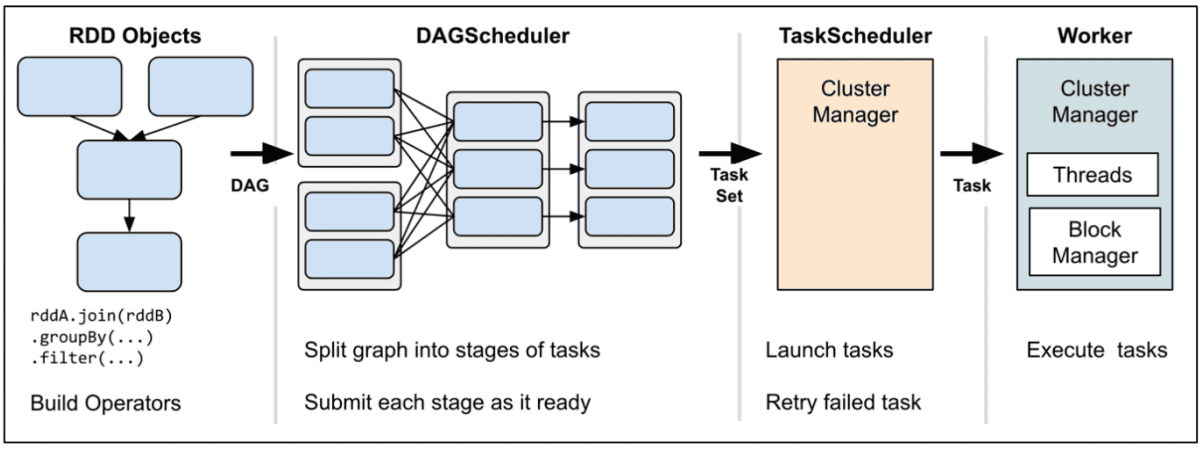
\includegraphics[width=\textwidth]{images/sparkapp.png}
		\caption{Spark app}
	\end{minipage}
\end{figure}
